%----------------------------------------------------------------------------------------
%	PACKAGES AND OTHER DOCUMENT CONFIGURATIONS
%----------------------------------------------------------------------------------------


\documentclass[12pt]{article}
\usepackage[english]{babel}
\usepackage[utf8x]{inputenc}
\usepackage{hyperref}
\usepackage{amsmath}
\usepackage{graphicx}
\usepackage[colorinlistoftodos]{todonotes}
\usepackage{eurosym}
\usepackage{listings}
\lstset{language=C}

\begin{document}

\begin{titlepage}

\newcommand{\HRule}{\rule{\linewidth}{0.3mm}} % Defines a new command for the horizontal lines, change thickness here

\center % Center everything on the page
 
%----------------------------------------------------------------------------------------
%	HEADING SECTIONS
%----------------------------------------------------------------------------------------

\textsc{\LARGE University of Auckland}\\[1.5cm] % Name of your university/college
\textsc{\Large CS760 Datamining and Machine Learning}\\[0.5cm] % Major heading such as course name
\textsc{\large Assignment 1}\\[0.5cm] % Minor heading such as course title

%----------------------------------------------------------------------------------------
%	TITLE SECTION
%----------------------------------------------------------------------------------------

\HRule \\[0.4cm]
{ \LARGE \bfseries Case-based reasoning - Travel Case}\\[0.1cm] % Title of your document
\HRule \\[1.5cm]
 
%----------------------------------------------------------------------------------------
%	AUTHOR SECTION
%----------------------------------------------------------------------------------------

\begin{minipage}{0.4\textwidth}
\begin{flushleft} \large
\emph{Author:}\\
Joel Glemne
\end{flushleft}
\end{minipage}
~
\begin{minipage}{0.4\textwidth}
\begin{flushright} \large
\emph{Student-id:} \\
145076454
\end{flushright}
\end{minipage}\\[2cm]

%\Large \emph{Author:}\\
%Joel Glemne\\
%\Large \emph{Student-id:}\\
%145076454\\[1cm]


%----------------------------------------------------------------------------------------
%	DATE AND LOGO
%----------------------------------------------------------------------------------------

{\large \today}\\[2cm] 

\includegraphics[width=4cm,height=4cm]{uoa-logo.png}\\[1cm] 
 
%----------------------------------------------------------------------------------------

\vfill % Fill the rest of the page with whitespace

\end{titlepage}


\begin{abstract}
This report was produced as part of a project in the course Datamining and Machine Learning at University of Auckland. The aim with the project was to examine how a case-based reasoner could be designed and implemented to produce an application able to give a user the possibilty to enter vacation preferences and then, based on previous experiences or \textit{cases} in the case-base, give the user vacation suggestions. 

The application was implemented with Python and PostgreSQL, using Tkinter, Geopy and Psycopg2. Retrieval algorithms used was standard brute force k-NN and a full footprint-based algorithm (FPRS) designed specifically for this project. \\\\There are several possible development areas. 

\begin{itemize}
\item The application assumes an adaptation method where the price feature is central but researching other ways to adapt the results would be preferable. 
\item When examining the region feature of all the cases, a geographical comparison is made using the coordinates. Some sort of association system containing e.g. tags would probably make similarity measurement even more adequate.
\item The application would not yet be considered to be in production mode, since the functionality of adding, editing and deleting cases only does so for class instances and not changes the database. That code is still hidden from the graphical user interface. 
\item This application was implemented by a complete Python-novice which makes it possible that the code has some inconsistencies and could probably be majorly improved considering speed and structure. 
\end{itemize}
\end{abstract}

\clearpage

\tableofcontents
\clearpage

\section{Introduction to CBR}
\label{sec:intro}

This section is divided into three sections; one giving an everyday life example with the purpose of giving an intuitive understanding of case-based reasoning (\textbf{CBR}), one section with a more theoretically general description followed by a mathematical description of the global similarity metrics. 

\subsection{Intuitive approach}
\label{sec:intuitive}

In your everyday life you meet many small problems that you probably would consider quite simple. Let us imagine that you are at your girlfriend's house for the first time, having dinner with his family. The mother asks you to go fetch one more plate. What do you do?

If it was me, I would first go to the kitchen. Then, I would start to look around if I see any \textit{obvious} place for the plates to be (be sure to notice the word \textit{obvious} for later). After that, I would start looking in the cabins. What is then funny, is that the possibility of me finding the right cabin on the first try would be high. How is that possible? 

The reason why, is that we often base our decisions on previous \textit{experiences} and the outcome of those experiences. I have been to a lot of kitchens before and it is common that different families - at least families from the same culture - organize their kitchens in similar ways. What I did, was simply evaluating (\textbf{reasoning}) my \textbf{base} of previous experiences (\textbf{cases}) in order to find a similar solution for the given problem. 

\subsection{General approach}
\label{sec:general}

CBR is mainly a technique for solving a large varieties of problems. Though, to fully understand the concept of CBR it is important to explain the meanings of \textit{case-base} and \textit{reasoning}.

A \textit{case-base} is a collection of experienced solutions to similar problems. \textit{Reasoning} is the procedure of drawing conclusions based on previous cases in order to solve a given problem. It is, however, important to note that it is not necessary to find an exact replica of the considered problem in order to find a solution, but only a \textit{similar} problem. What is then important in the CBR methodology is how to decide what \textit{similar} means. 

In the example in section 1.1 the word \textit{obvious} was used. What obvious means is basically that the given case problem is very similar to a, or several, previous experienced case(s). For humans, it might seem easy to compare different cases and identify all key \textit{features} in an instant, but for a computer it is crucial to pre-identify key features, define and assign similarity metrics to each feature and then organize everything into a reusable model for comparing different cases and predict outcome. \cite{cbr}

\subsection{Mathematical approach}
\label{sec:math}

The similarity between two cases is calculated according to the k-nearest neighbors algorithm explained here below. \\\\
Assume a case-base of $n$ cases $y_i$ where $i=1,2,...\,,n$ and each case having the same $m$ pre-defined features with different values. For each feature a \textit{local} similarity function $sim_j$ is defined where $j=1,2,...\,,m$. The functions takes two arbitrary cases $a,b$ as arguments so that $0 \leq sim_j(a,b) \leq 1$. Every feature is also assigned a weight $\omega_j$ which corresponds to the \textit{local} simililarity's importance to the \textit{global} similarity. 

When comparing an arbitrary \textbf{target case} $x$ with all the \textbf{source cases} in the assumed case-base, $n$ \textit{global} similarities $S_i$ are produced where $0 \leq S_i \leq 1$. $S_i$ is defined as $$S_i=\frac{s_i}{W}$$ where $$s_i=\sum_{1}^{j=m} (\omega_j * sim_j(x,y_i))$$ and $$W=\sum_{1}^{j=m}\omega_j$$
In order to find the most similar cases in the case-base, the cases $y_i$ corresponding to the highest global similarities $S_i$ are chosen. \cite{cbr}

One of the most interesting things in this algorithm is how the local similarity functions $sim_j$ are defined individually. This is what is handled in the next section of this report. 

\clearpage

\section{Features}
\label{sec:features}

In this section, all the local similarity functions for the given case-base are presented and motivated. 

As described in section 1.3, every case has a couple of pre-defined \textit{features} or \textit{variables}. In this application the cases considered are different options for travel plans and they all have the following features:

\begin{enumerate}
\item Accommodation
\item Case name
\item Duration
\item Holiday type
\item Hotel
\item Journey code
\item Number of persons
\item Price
\item Region
\item Season
\item Transportation
\end{enumerate}

Every feature has its own local similarity function, producing values within a range of $[0,1]$, and an assigned weight within the range $[1,\infty[$. If a feature is considered important for the global similarity calculation, it is assigned a high value and vice versa. 

\subsection{Accommodation}
\label{sec:accommodation}

The possible values for the accommodation feature were: 

\begin{enumerate}
\item HolidayFlat
\item OneStar
\item TwoStars
\item ThreeStars
\item FourStars
\item FiveStars
\end{enumerate}

\subsubsection{Local similarity function}
\label{sec:acc-sim}

To calculate the local similarity of accommodation between two arbitrary cases, some sort of ranking was here needed. 
In this case, HolidayFlat was considered the least exclusive kind of accommodation and thereafter rising with number of stars. All of the feature values were therefore assigned an integer value $I_{acc}$ corresponding to above given table numbers, e.g. for an arbitrary case $a$ which has the feature value TwoStars, $I_{acc}(a)=3$. 

In order to produce a similarity $sim_{acc}$ so that $0 \leq sim_{acc} \leq 1$, it was here assumed a \textit{more-is-perfect} approach with a linear calculation of the similarity. This means, that if $I_{acc}(target\,case) \leq I_{acc}(source\,case)$, then $sim_{acc}=1$. Otherwise, the similarity is calculated as $$sim_{acc}=\frac{range-(I_{acc}(target\,case)-I_{acc}(source\,case))}{range}$$
where $range=6-1=5$. \cite{cbr}

\subsubsection{Feature weight}
\label{sec:acc-weight}

When considering a vacation option, the accommodation type is normally considered a feature which gives an extra bonus to the experience rather than being a feature vital for the selection. Therefore, the accommodation feature is given a relatively low weight  $\omega_{acc}=3$. 

\subsection{Case name}
\label{sec:case-name}

Since the case name by definition is unique for each case, e.g. \textit{Journey984}, and really does not give any information about the case, this feature is not considered in the similarity metrics. It is however interesting to save it in the database since it is then very easy to search for the given case.

\subsection{Duration}
\label{sec:duration}

Duration of a vacation is most of the time adjusted according to the number of vacation days you are given by your employer, which makes this feature quite important for the selection of vacation. The more interesting discussion is rather how adaptable this feature is, a discussion more thoroughly dealt with in an own section here below; \textit{Adaptation discussion}.

\subsubsection{Local similarity function}
\label{sec:dur-sim}

If the duration in the given target case, $D(target\,case)$, is exactly the same as the one in the source case, $D(source\,case)$, the similarity $sim_{dur}$ is set equal to 1. For other source cases, where the difference between the compared cases durations are less than or equal to 5, the similarity is calculated as: $$sim_{dur}=\frac{5-(D(target\,case)-D(source\,case))}{5}$$
For cases where the difference is larger than 5 days, $sim_{dur}=0$.

\subsubsection{Feature weight}
\label{sec:dur-weight}

Since this feature is considered to be adaptable, the feature is given a correspondingly low weight of $\omega_{dur}=2$. 

\subsubsection{Adaptation discussion}
\label{sec:dur-adapt}

In this application, it is supposed that the duration could be adapted by the accommodation provider but that is rather reflected in how the price similarity is calculated. For more info, see Section \ref{sec:price}. 

\subsection{Holiday type}
\label{sec:ht}

The holiday type has a couple of different possible values, all given in one of the lecture slides. In this application all these different types are entered into a taxonomy tree according to Figure~\ref{fig:taxonomy-tree-ht.png} here below.

\begin{figure}[h]
\centering

\includegraphics[width=1\textwidth]{taxonomy-tree-ht.png}
\caption{\label{fig:taxonomy-tree-ht.png}Taxonomy tree for holiday types}
\end{figure}

\subsubsection{Local similarity function}
\label{sec:ht-sim}

What the tree says, is that if you for example are comparing \textit{Diving} with \textit{Surfing}, the similarity will be equal to $0.5$, but if you are comparing \textit{Diving} with for example \textit{Shopping} or any other feature value outside of the same group, the similarity will be $0.3$.

\subsubsection{Feature weight}
\label{sec:ht-weight}

With the exception of hotel name and journey code, holiday type is in this program considered to be the most important feature and is given the high value $\omega_{ht}=10$. The reasoning behind this is that one normally first consider what the purpose or main activity during the trip will be and then consider place and everything else. These assumptions are based on personal common knowledge and very informal interviews with friends. 

\subsection{Hotel}
\label{sec:hotel}

This feature is simply the name of the hotel given in the case. 

\subsubsection{Local similarity function}
\label{sec:hotel-sim}

Since the hotel names really does not say anything about the standard of the hotel or any other features, this is considered a fairly unimportant feature for one who considers different options for a vacation and does not have a certain hotel in mind. That is why if the exact hotel name is entered, then the similiarity will be equal to 1, otherwise it will be equal to 0. 

\subsubsection{Feature weight}
\label{sec:hotel-weight}

Would the case be that one has heard that a certain hotel is considered to be really good or if one has stayed at a certain hotel before, than perhaps it is likely that the hotel name will be requested. Would that be the case, it certainly should be prioritized when actually entering the name of the hotel. It has therefore been given the high weight $\omega_{hotel}=20$. 

\subsection{Journey code}
\label{sec:jc}

The journey code is only an integer, mostly used as an id of the case. Would the case be that one is searching for a specific case, the similarity will be 1 if the query is the same, otherwise it will be 0. Since this only would be used to find a single certain case, the weight is assigned the extreme value $\omega_{jc}=200$, just to be sure that the certain case is found. This feature is however not included in the GUI since this is not considered a preference of a vacation. 

\subsection{Number of persons}
\label{sec:nop}

The feature \textit{Number of persons} is exactly what it sounds like. This is most of the time something that is not really adjustable \textit{for the customer} when considering different vacation options, but it is at many hotels adaptable so that it may suit the customer. As said before, the thing one really is looking for is the price per person per day. This will be covered in Section \ref{sec:price}. 

\subsubsection{Local similarity function}
\label{sec:nop-sim}

The similarity for number of persons is calculated in the exact same way as the duration. 

\subsubsection{Feature weight}
\label{sec:nop-weight}

With the same reasoning as with duration, weight also here is set to $\omega_{nop}=2$. 

\subsection{Price}
\label{sec:price}

Price is the total cost for an arbitrary vacation, in this application evaluated as in the currency Euro (\euro).

Price is the feature which in this application sort of decides the adaptation of a certain case. The similarity function is therefore desgined accordingly.

\subsubsection{Local similarity function}
\label{sec:price-sim}

The similarity function for price depends on whether the user has entered duration and/or number of persons in addition to the requested price. Depending on which, a similarity measure is made with a price equal to either of these four cases:

\begin{itemize}
\item Total price - neither number of persons nor duration were entered
\item Price per person - only number of persons was entered
\item Price per day - only duration was entered
\item Price per person per day - both duration and number of persons were entered
\end{itemize}

With this said, the similarity was then calculated with a simple linear function. Since the lower limit of the price range ($[239,8007]$) in the given case base was close to zero, it was considered redundant and in practice set to zero. The reason why was that this program assumes that if someone e.g. enters the value $0$ as price, the presumable goal is to find the lowest possible price. 

Therefore, the similarity, $sim_{price}$, was calculated with a \textit{less-is-perfect} model, where $sim_{price}=1$ if the price difference $diff_{price}=Price(source \, case) - Price(target \, case) \leq 0$ and otherwise as: $$sim_{price}=\frac{range_{price} - diff_{price}}{range_{price}}$$ where $range_{price}=8007$ with respect to above given argumentation. \cite{cbr}

\subsubsection{Feature weight}
\label{sec:price-weight}

Price was considered an important feature and an important topic to discuss when talking about adaptation, see Section \ref{sec:price-adapt} for more on adaptation. Price was here given the high weight value $\omega_{price}=9$.

\subsubsection{Adaptation discussion}
\label{sec:price-adapt}

Since duration, number of persons and price were evaluated as the most adaptable features in these cases, one could argue how these should be adapted and correlated to one another. The conclusion in this assignment was that it all eventually boils down to the price and that the price therefore should be the deciding argument of the three, still decided with the other adaptable features as arguments. 

\subsection{Region}
\label{sec:region}

The region solely contained the information of geographical location. The feature was considered a very hard feature to design a similarity function for and therefore demands a more thorough discussion.

\subsubsection{Discussion}
\label{sec:region-discussion}

A region can have many different characteristics and a taxonomy tree or similar would be enormous and not very agile. It is also noticeable that a seemingly endless list of new regions can be added. 

Because of this, since a quite large amount of different regions were given in the case-base and it was evaluated that scalability is preferable, the program uses the Google Maps to find coordinates for the region and then compares different regions based on distance and difference in latitude. The reason why latitude and not longitude was chosen as a deciding parameter was that people most commonly aims for a certain climate and the climate is much more dependent on latitude than longitude. 

The similarity function for the region is, however, a feature which could be much more thoroughly discussed and evaluated. One could argue that some sort of association system could be used where each location is given a tag based on the characteristics of the region. Presumably there could be a number of given tags which are all assigned individually to each region and through them then connected with similar regions. 

This program was in some way a prototype and a development opportunity could certainly be to add some sort of association system for all the regions to the existing similarity function, perhaps altering the importance weight for the global similarity measure. 

\subsubsection{Local similarity function}
\label{sec:region-sim}

With reference to above discussion, the similarity, $sim_{region}$, was calculated as a linear function depending on geographical distance and difference in latitude. If the region for the target case is the same as the region in the source case, then $sim_{region}=1$. If that is not the case, there are two different possibilities. If the distance is evaluated as more than $2000$ km then $sim_{region}=0$. Otherwise, a similarity is calculated with respect to the distance and the latitude difference - with a higher weight given to the latitude difference - much in the same way as previous linear calculations. 

\subsubsection{Feature weight}
\label{sec:region-weight}

With the discussion in mind, that the feature was hard to adequately compare, meaning that the comparison could be excluding important measurements, this feature is given a reasonably low weight of $\omega_{region}=2$. 

\subsection{Season}
\label{sec:season}

The season values was given as all the months of a year. 

\subsubsection{Local similarity function}
\label{sec:season-sim}

The solution here was to assign each month a new \textit{season}: 

\begin{itemize}
\item Winter - December, January, February
\item Spring - March, April, May
\item Summer - June, July, August
\item Autumn - September, October, November
\end{itemize}

and then calculate the similarity, $sim_{season}$, with four possible values:

\begin{itemize}
\item 1 - if the month is the same in both target case and source case
\item 0.5 - if the months are in the same \textit{season}
\item 0.2 - if the months are \textit{neighbors} but are not in the same \textit{season}, e.g. June and May.
\item 0 otherwise
\end{itemize}

\subsubsection{Feature weight}
\label{sec:season-weight}

In this assignment, season was evaluated as a quite important feature, since it is common that one not independently chooses when going for vacation. Instead, the most common case is normally that many factors around are at hand and therefore gives low flexibility to change the period of the vacation (employer, family and friends vacation times etc.). It was therefore given a weight $\omega_{season}=5$.

\subsection{Transportation}
\label{sec:transport}

Transportation has four possible values: \textit{Car}, \textit{Plane}, \textit{Coach} or \textit{Train}. 

\subsubsection{Local similarity function}
\label{sec:transport-sim}

To compare these alternatives of transportation, a decision table was made within the application, which can be viewed in Table~\ref{tab:transport}. 

\begin{table}[h]
\centering
\begin{tabular}{l|cccc}
  & Car & Coach & Plane & Train\\\hline
Car & 1 & 0.5 & 0.2 & 0.8 \\
Coach & 0.5 & 1.0 & 0.0 & 0.7 \\
Plane & 0.0 & 0.0 & 1.0 & 0.0 \\
Train & 0.3 & 0.7 & 0.0 & 1.0
\end{tabular}
\caption{\label{tab:transport}Decision table for transportation}
\end{table}

The decision table was taken almost entirely from one of the lecture slides, with some adjustments motivated here below:

\begin{itemize}
\item Car - chosen when looking for convenience, freedom and a somewhat affordable option. See motivations below:
\begin{itemize}
\item Coach
\subitem Less freedom - sitting still and almost no ability to choose spontaneous stops - but you are still choosing an affordable option and there are often several pre-defined stops during the way. Similarity $sim_{transport}=0.5$
\item Plane
\subitem Almost no freedom and could be pricy - but there is a little upside of possibly getting extra time. $sim_{transport}=0.2$
\item Train
\subitem More inside freedom, (possibly) more comfortability than with a car and still pretty affordable. However, there is zero possibility to invoke spontaneuos stops.
\end{itemize}
\item Coach - chosen when looking for an affordable option and no obligations of having a car. Still a little freedom of jumping off at several stops. 
\begin{itemize}
\item Car
\subitem Similar discussion as with Car-Coach but reversed. $sim_{transport}=0.5$
\item Plane
\subitem Similar discussion as with Car-Plane but price difference is most of the time even higher and you lose the upsides of bus. Plane is also considered an environmentally unfriendly choice. $sim_{transport}=0.0$
\item Train
\subitem Pretty similar to bus in many ways. $sim_{transport}=0.7$
\end{itemize}
\item Plane - very specific choice and when wanting to fly, one really does not want any other choice. All similarities other than Plane-Plane: $sim_{transport}=0.0$.
\item Train - refers to above discussion. 
\end{itemize}

\subsubsection{Feature weight}
\label{sec:transport-weight}

Transportation is mostly something that is decided beforehand but can still be changed if the rest of the vacation fits most of the requirements. Therefore the weight is $\omega_{transport}=4$.

\clearpage

\section{Retrieval algorithm}
\label{sec:retrieval}

In order to make the program scalable, a PostgreSQL database \textit{travel} was created to store the information about all the cases. In the database there are two tables, \textit{cases} and \textit{regions}. A further description of the database can be found in the appendix. 

All the cases were loaded into the database and functionality is prepared for adding more cases to the database either individually or as a collection (either as an excel-file or an ASCII-file). 

Whenever all the cases are retrieved, they may be retrieved with the usage of two different algorithms: \textit{brute force k-NN} (default) or \textit{full footprint-based approach} (FPRS). 

\subsection{Brute force k-NN}
\label{sec:knn}

Whenever a target case is presented to the application, the target case is compared with all source cases. The best results are then presented as a list in the user interface. 

\subsection{Full footprint-based approach (FPRS)}
\label{sec:fprs}

The theory behind FPRS is to choose a couple of key cases that each has their own smaller case-base which is a fraction of the entire case-base. The key cases are chosen based on the similarity distance between the source cases, see Figure~\ref{fig:fprs-1.png}.\cite{lect}

\begin{figure}[h]
\centering
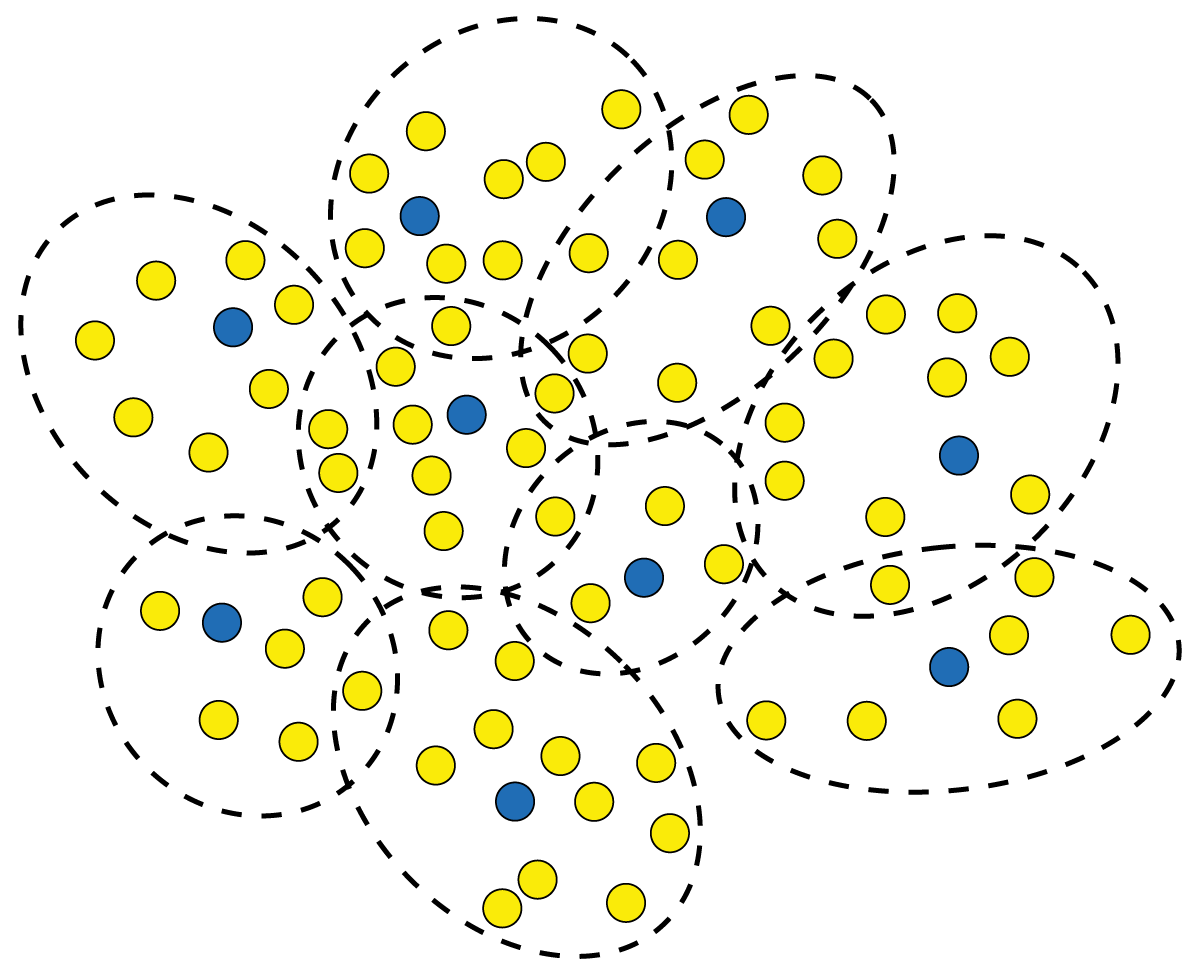
\includegraphics[width=0.7\textwidth]{fprs-1.png}
\caption{\label{fig:fprs-1.png}The blue spots represents the key cases and the yellow spots represents all the source cases. As seen in the figure, all the source cases are sorted into groups consisting of one key case and a bunch of source cases. When using FPRS, the target case is first compared with all the key cases and only the source cases in the groups containing the most similar key cases will then be compared with the target case.}
\end{figure}

Then, whenever a target case is presented to the application, the target case is first compared with all the key cases and then compared with the source cases connected to the key cases where the similarity is the highest. Those cases with the highest similarities will be presented in the GUI-list. 

It is in the user interface possible to choose number of key cases that will be considered during the comparison. For example, as a default this number is set to 6. This means that the 6 key cases that has the highest similarity with the target case will be compared with the target case as well as all the source cases connected to those 6 key cases. 

This means that if fewer key cases are considered, the possibility of finding the most similar case will be lower but the number of cases compared will be considerably less and therefore improve the speed of the application. 

\clearpage

\section{Implementation}
\label{sec:implementation}

\subsection{Language and tools}
\label{sec:language}

Python v3.4.3 was chosen as the language and PyCharm v2016.1.4 as the environment for the assignment. The reason was because the author had never used neither of those before and wanted to learn something new. The code might therefore contain some inconsistencies since different means of solving similar problems were discovered throughout the implementation. 

As mentioned before, PostgreSQL v9.5.1 was used to create a database for storing all the information about the cases, but pretty much all the code is written in Python using Psycopg2 as a database adapter for connecting with the database through the application. The reason for using a database was that it would be easy to scale up the application and adding new information.

In order to categorize the different regions, the application uses the Python library geopy, which is a geocoding library connecting with Google Maps to get geographical information about certain places. 

For GUI, the application uses the standard Python package Tkinter. 

\subsection{File and class structure}
\label{sec:files}

There are five files in the application that were used: \textit{main.py}, \textit{tools.py}, \textit{features.py}, \textit{setup.py} and \textit{globals.py}. The code in setup.py is not used at the moment but contains code for extracting cases from ASCII- or Excel-files. The most important classes of the application are here listed.

\begin{itemize}
\item TargetCase
\begin{itemize}
\item The class which gives the structure and methods for the instances of target cases. TargetCase is the superclass for SourceCase and is found in main.py. 
\end{itemize}
\item SourceCase
\begin{itemize}
\item The class which gives the structure and methods for the instances of source cases. Inherits the class TargetCase and is also found in main.py. Every instance of SourceCase always points to the target case at hand. All instances of TargetCase and SourceCase points to instances of feature classes containing information about all the features. These feature classes are found in features.py. Speaking of similarity metrics, this is where most of the interesting code is. 
\end{itemize}
\item App
\begin{itemize}
\item This class works as the application interface and refers to instances of other help classes CaseList, Field, DropDown and Menu to organize the GUI. The entire application is started during the creation of the App instance. 
\end{itemize}
\end{itemize}

\clearpage

\section{Interface}
\label{sec:interface}

When running the program, the window in Figure~\ref{fig:start-page.png} is shown. 

\begin{figure}[h]
\centering
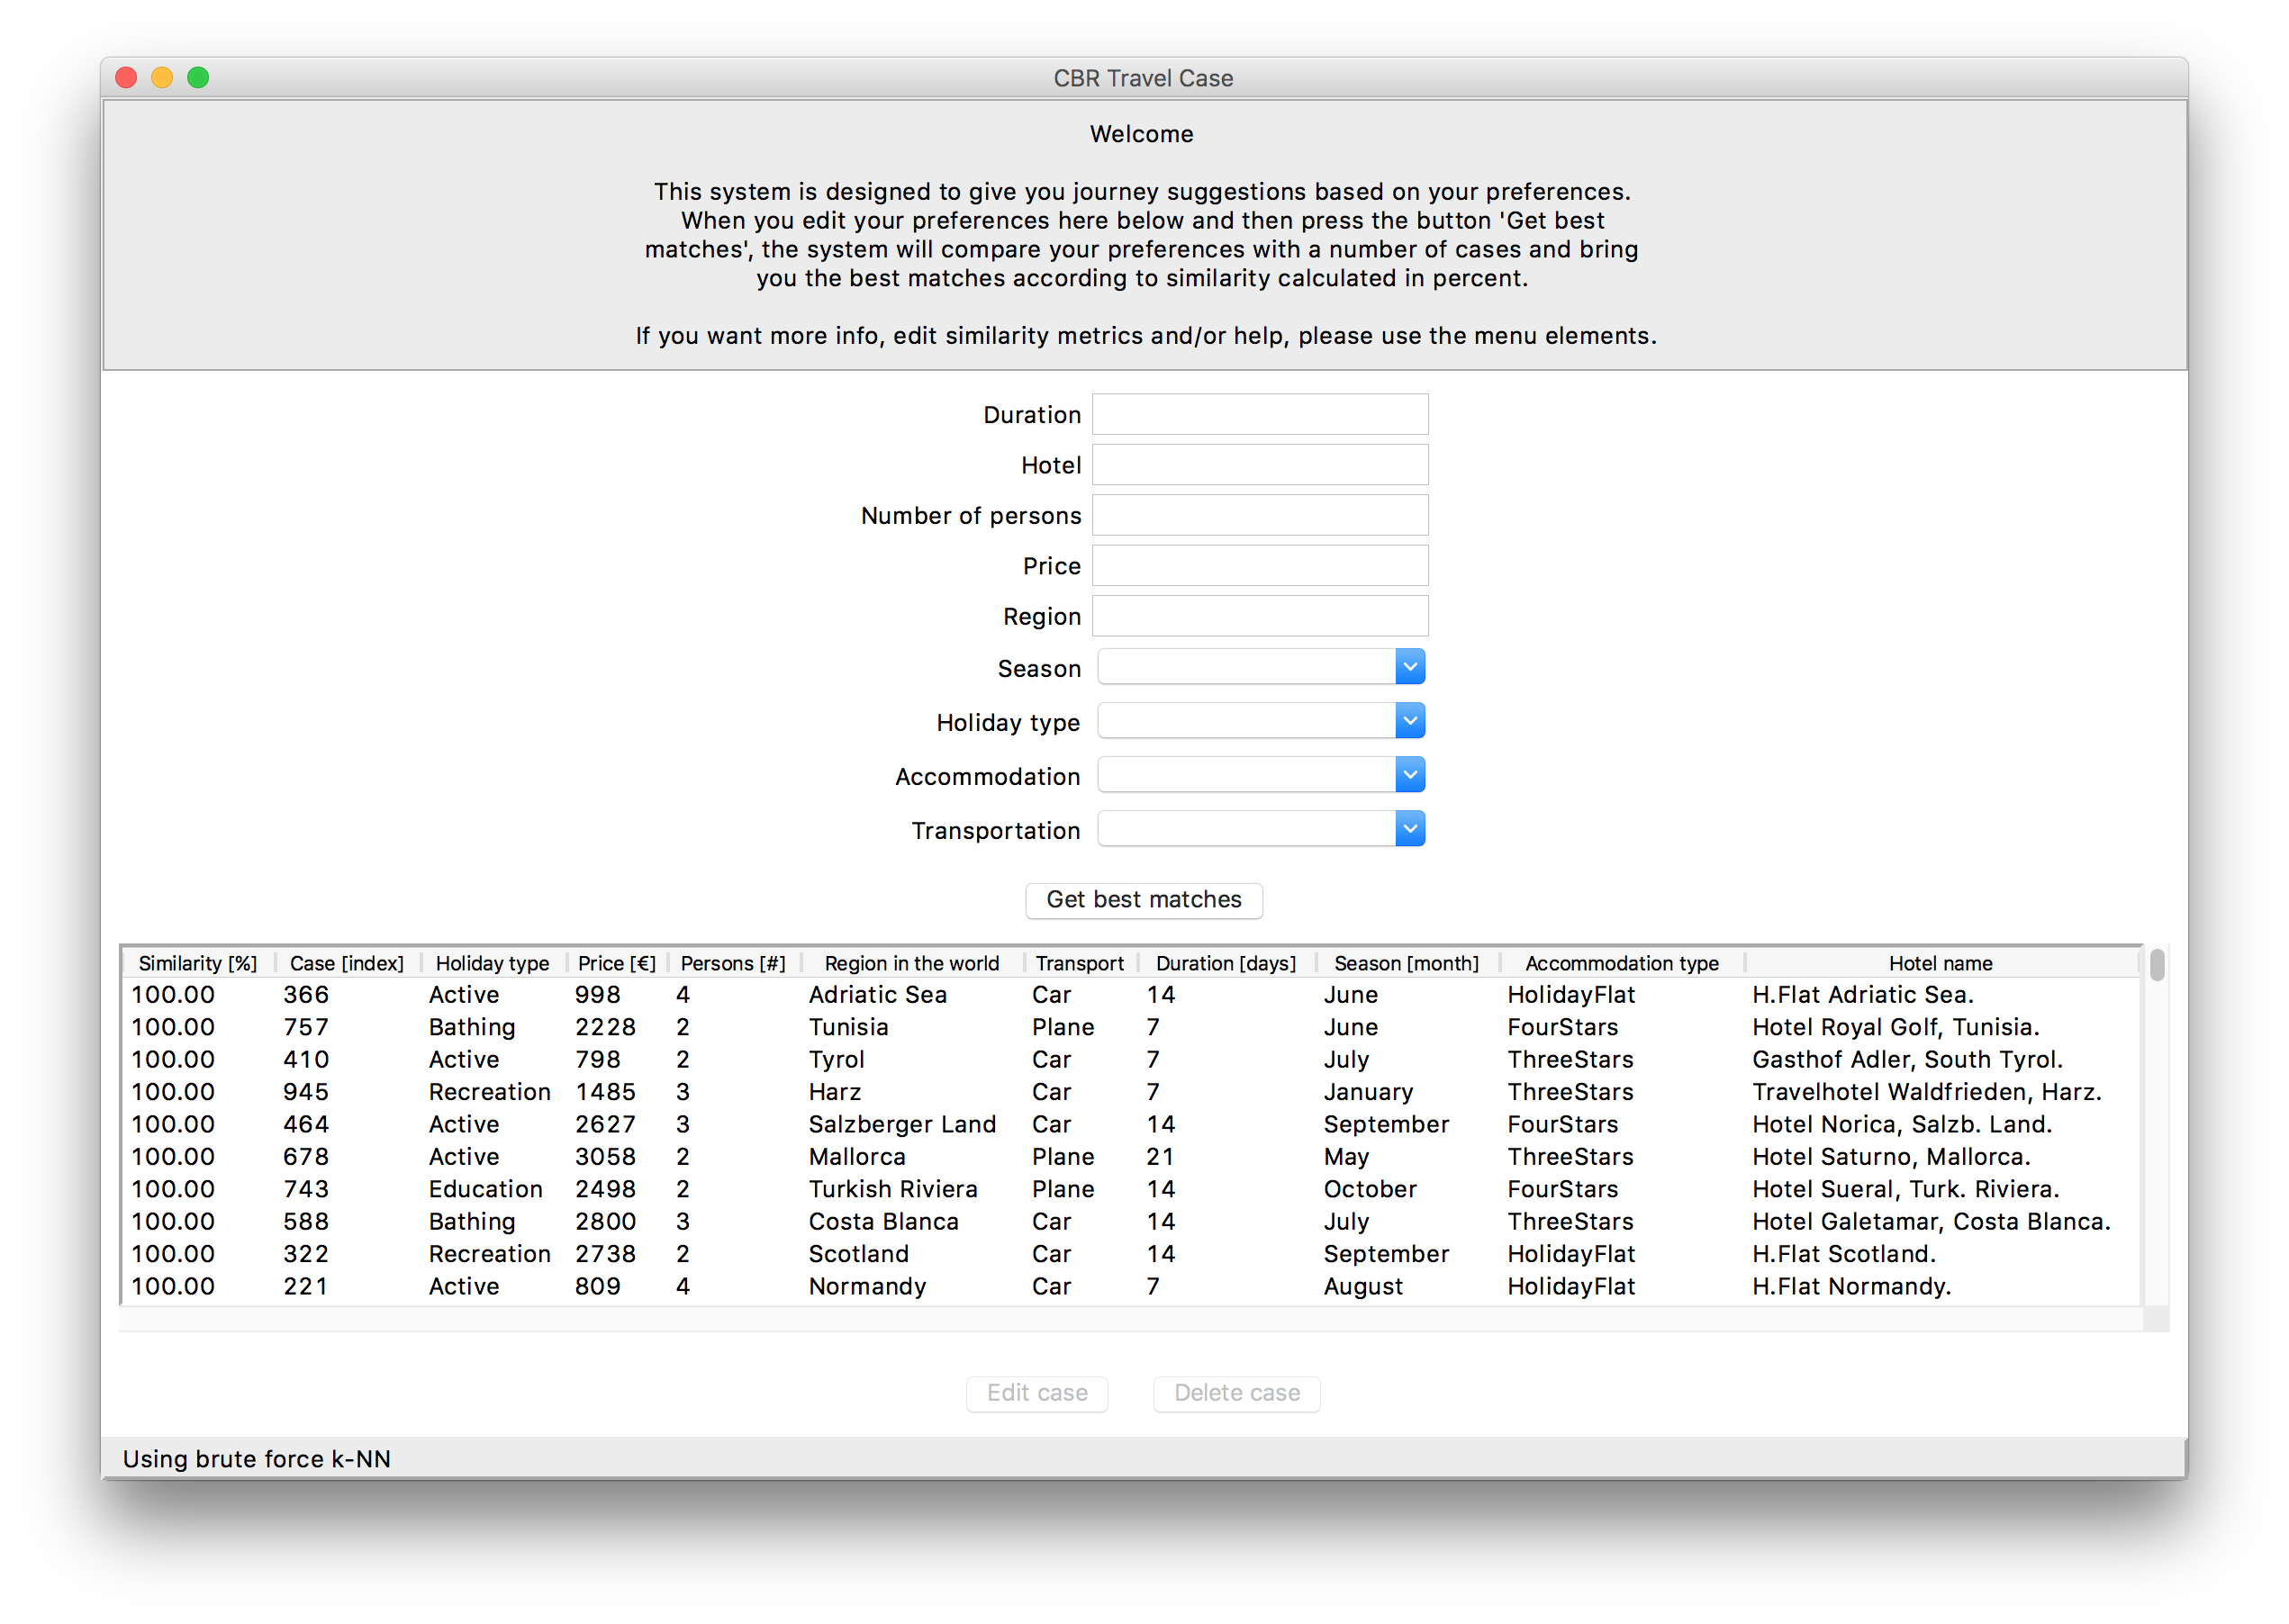
\includegraphics[width=1\textwidth]{start-page.png}
\caption{\label{fig:start-page.png}Start page}
\end{figure}

The user is given the opportunity to enter different preferences according to the given fields and dropdowns. When pressing the button \textit{Get best matches}, the comparison begins. The preferences entered makes up a target case that will be compared with the source cases to find the best matches. When the comparison is finished, the list is filled with all the best matches. 

The list contains all information about the cases sorted into seperate columns. The cases are automatically sorted by the similarity (viewed as a percentage) but if the user would like to sort the cases by other columns it is possible to do so by simply pressing the header column corresponding to the column the user wishes to sort by. 

\subsection{Extra features}
\label{sec:extra}

There are some extra features included in the application. If the user wants to change the weights associated with each case feature, one can do so by pressing the menu element \textit{Similarities} and then choose the dropdown button \textit{Edit weights}. 

\begin{figure}[h]
\centering
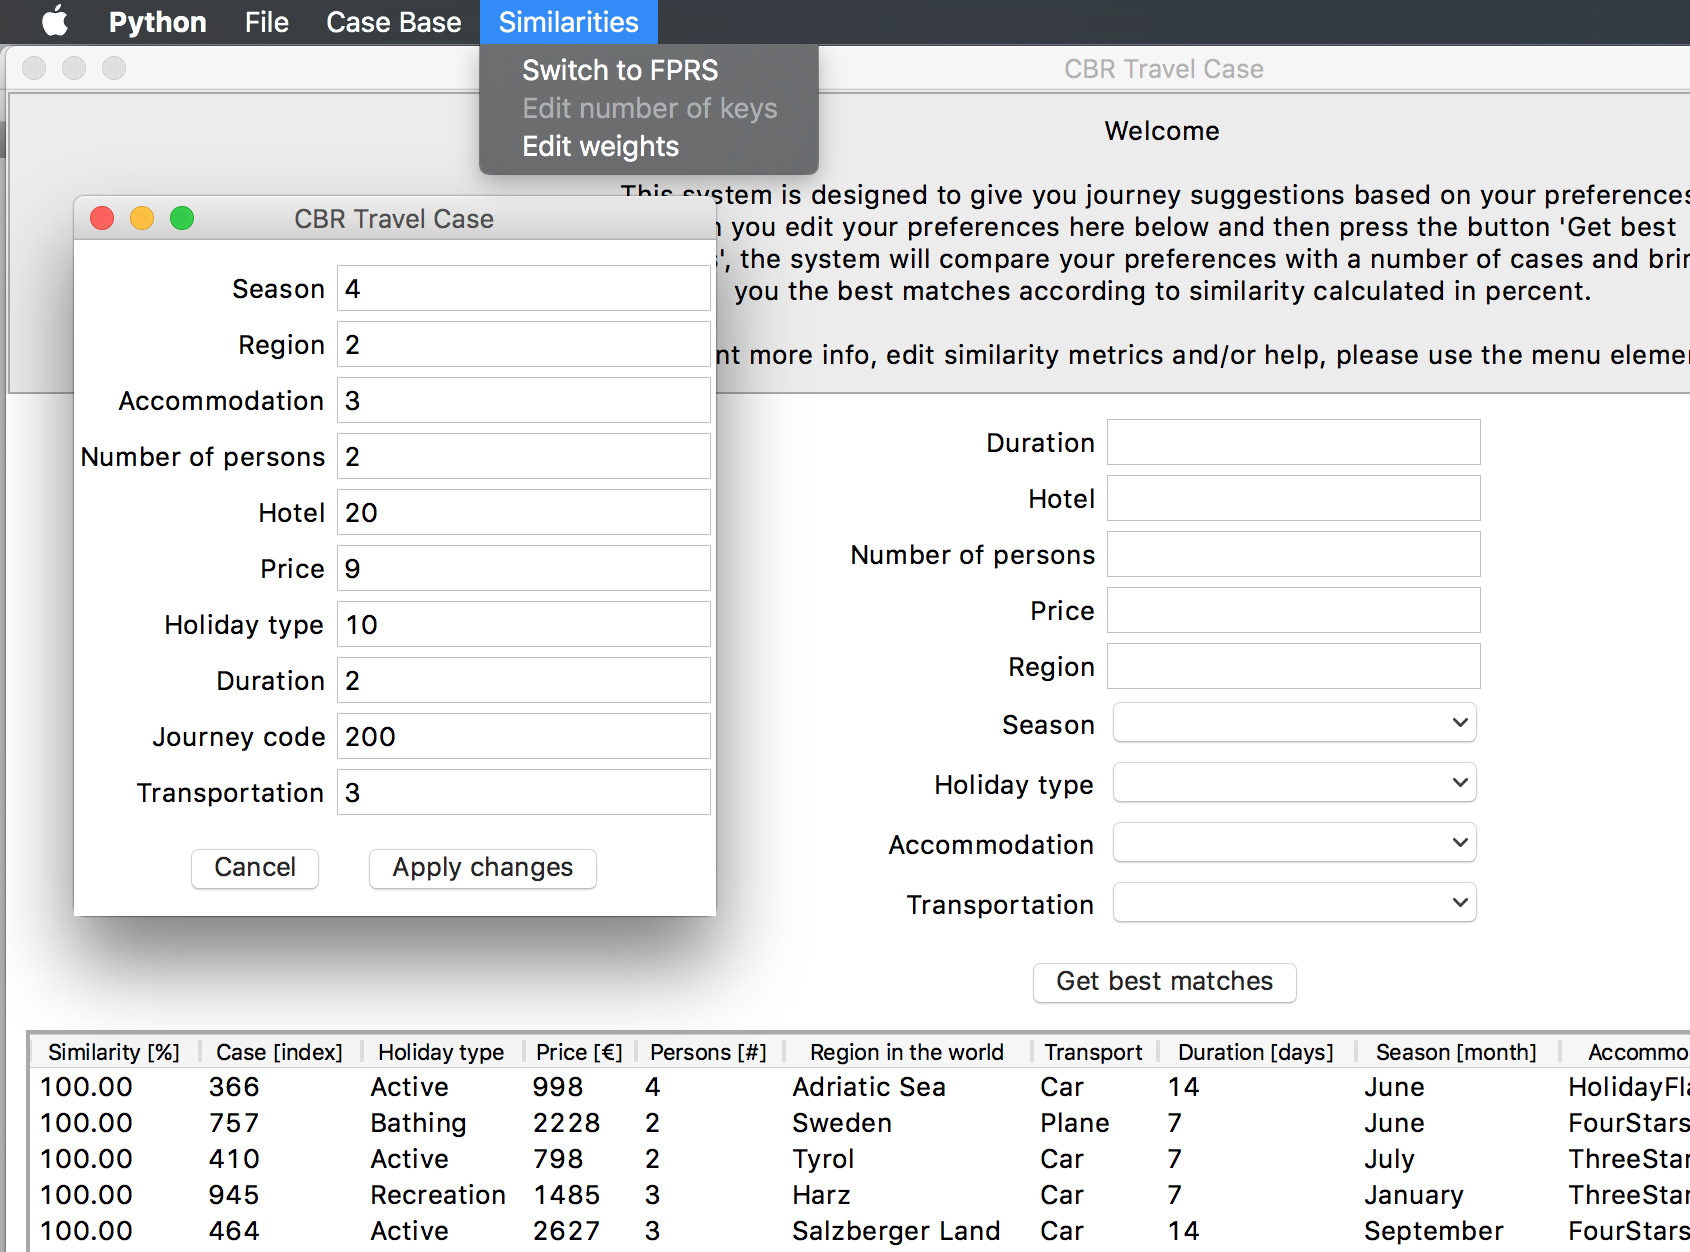
\includegraphics[width=0.8\textwidth]{edit-weights.png}
\caption{\label{fig:edit-weights.png}Edit weights}
\end{figure}

A new window is then opened with the current weight values and the possibility to change them as shown in Figure~\ref{fig:edit-weights.png}.

Another feature is that if the user wants to add, edit or delete a case it is possible by selecting a certain case in the list and then using the menu elements in the same way as with changing the feature weights. 

If the user wants to switch retrieval algorithm, it is also possible by using the menu elements. Which algorithm is currently used is shown in the status bar at the bottom. When using FPRS it is also possible to change number of key cases considered during the retrieval in order to make the retrieval faster or more accurate. 

\clearpage

\section{Installation and running program}
\label{sec:install}

The program has been tested on a Mac OS X v10.11.6 with Python v3.4.3 and PostgreSQL v9.5.1. To be able to run the program the user first needs to install PostgreSQL, geopy and psycopg2. Using homebrew and pip3, installation can be done with these commands in the terminal:

\begin{lstlisting}
$ brew install postgresql
$ pip3 install geopy
$ pip3 install psycopg2
\end{lstlisting}

When that is done, the database server program \textit{postgres} needs to be started. This is done with:

\begin{lstlisting}
$ postgres -D /usr/local/var/postgres
\end{lstlisting}

The location should be where the file \textit{postgresql.conf} is located. That will leave the server running in the foreground so it is important to leave that tab of the terminal open and open a new one to restore the database. Navigate to the folder where the source files are located and especially where the file \textit{traveldb.dump} is. To restore the database, use following command:

\begin{lstlisting}
$ pg_restore -C -d postgres traveldb.dump
\end{lstlisting}

When that is done, the program can be started with:

\begin{lstlisting}
$ python3 main.py
\end{lstlisting}

If there for some reason would be any problem with restoring the database with above given command, the database is created from scratch with commands given here below, given that there exists no database with the name "travel".

\begin{lstlisting}
$ createdb travel
$ psql travel
travel=# CREATE TABLE IF NOT EXISTS "cases" (
	"id" SERIAL PRIMARY KEY,
	"case_name" varchar(20),
	"journey_code" int,
	"holiday_type" varchar(20),
	"price" int,
	"number_of_persons" int,
	"region" varchar(80),
	"transportation" varchar(20),
	"duration" int,
	"season" varchar(20),
	"accommodation" varchar(30),
	"hotel" varchar(80)
);
travel=# CREATE TABLE IF NOT EXISTS "regions" (
	"id" SERIAL PRIMARY KEY,
	"region_name" varchar(80),
	"latitude" float,
	"longitude" float
);
\end{lstlisting}

To then load all the cases to the database, just run this in another terminal tab:

\begin{lstlisting}
$ python3 setup.py
\end{lstlisting}

When this is done, the program can be run in the same way as before:

\begin{lstlisting}
$ python3 main.py
\end{lstlisting}

\clearpage

\begin{thebibliography}{9}

\bibitem{cbr}
Michael M. Richter \& Rosina O. Weber,
\emph{Case-Based Reasoning},
Springer-Verlag Berlin Heidelberg,
2013.

\bibitem{lect}
Ian Watson,
\emph{Lecture notes CS760},
University of Auckland,
2016


\end{thebibliography}

\end{document}